\documentclass{report}

\PassOptionsToPackage{square, numbers}{natbib}
\usepackage{pgfplots}
\pgfplotsset{compat=1.18}
\usepackage[preprint]{neurips_2022}

\usepackage[utf8]{inputenc} % allow utf-8 input
\usepackage[T1]{fontenc}    % use 8-bit T1 fonts
\usepackage{hyperref}       % hyperlinks
\usepackage{url}            % simple URL typesetting
\usepackage{booktabs}       % professional-quality tables
\usepackage{amsfonts}       % blackboard math symbols
\usepackage{nicefrac}       % compact symbols for 1/2, etc.
\usepackage{microtype}      % microtypography
\usepackage{xcolor}         % colors
\usepackage{graphicx}
\usepackage{minted}

% % Sumit's package list
\usepackage{amsmath}
\usepackage{amssymb}
\usepackage{amsthm}
\newtheorem{theorem}{Theorem}[section]
\newtheorem{corollary}{Corollary}[theorem]
\newtheorem{lemma}{Lemma}[theorem]
\theoremstyle{definition}
\newtheorem{definition}{Definition}[section]
\newcommand{\E}{\mathop{\mathbb{E}}}
\renewcommand{\P}{\mathop{\mathbb{P}}}
\newcommand{\Var}{\operatorname{Var}}
\newcommand{\Cov}{\operatorname{Cov}}
\newcommand{\Corr}{\operatorname{Corr}}
\newcommand{\T}{\intercal}
\newcommand{\arrow}[0]{\xrightarrow{}}
\newcommand{\R}[0]{\mathbb{R}}
\newcommand{\N}[0]{\mathbb{N}}
\newcommand*\diff{\mathop{}\!\mathrm{d}}
\newcommand*\Diff[1]{\mathop{}\!\mathrm{d^#1}}
\newcommand\bigfrac[2]{\frac{\displaystyle #1}{\displaystyle #2}}
\def\bigo{\mathcal O}
\def\floor#1{\left\lfloor#1\right\rfloor}
\def\ceil#1{\left\lceil#1\right\rceil}
\def\norm#1{\left\lVert#1\right\rVert}
\def\iprod#1#2{\left\langle#1,#2\right\rangle}
\usepackage{enumitem}
\usepackage{color}
\usepackage{listings}
\usepackage{algorithm}
\usepackage{algpseudocode}
\usepackage[edges]{forest}
\usepackage{pgfplots}
\usepackage{adjustbox}
\usepackage{xstring}
\usepackage{ifthen}
\usetikzlibrary{positioning}
\usepackage{stmaryrd}


\title{BUFN403 Project Report}
\author{%
  Sumit Nawathe \quad Ravi Panguluri \quad James Zhang \quad Sashwat Venkatesh \\
  Computational Finance Minor Capstone \\
  University of Maryland College Park \\
  \texttt{\{snawathe, rpangulu, jzhang72, sashvenk\}@terpmail.umd.edu} \\
}

\begin{document}
\maketitle

\begin{abstract}
  We aim to create a reinforcement learning agent that utilizes historical price data
  as well as sentiment and topical embeddings of news articles to optimally trade on
  S\&P100 stocks. After implementing multiple papers on financial reinforcement learning
  for equity trading, our contribution will be in experimenting and synthesizing an improved
  combination of the state space and reward function for our environment. We compare our
  best strategy against other standard equity portfolio benchmarks.
\end{abstract}

\tableofcontents

\chapter{Project Overview}

\section{Introduction}

Our group is seeking to develop a reinforcement learning agent to support portfolio 
management and optimization. Utilizing both empirical stock pricing data along with 
alternative data, we look to create a more well-informed portfolio optimization tool. 

Our primary motivations for pursuing a reinforcement learning-based approach are as 
follows:

\begin{enumerate}
    \item Reinforcement learning lends itself well to learning/opening in an online environment. The agent can interact with its environment, providing real-time feedback/ responsiveness to allow for better results.
    \item Our approach involves incorporating alternative data to support the agent’s decision making process. Encoding this alt-data into the states matrix of the agent allows for the agent to make better decisions when it comes to adjusting portfolio weights.
    \item Given that a reinforcement learning agent’s decisions are modeled by a Markov Decision Process, we can easily provide different reward functions to account for a variety of investor preferences or restrictions.
\end{enumerate}



\section{Dataset Creation}

Creating a combined dataset encompassing a textual corpus sufficient for us to build 
a robust reinforcement learning agent will require pulling data from a wide variety 
of sources. We aim to use two primary types of data: stock and news data.

\subsection{Stock Data}

We retrieve data from Wharton Research Data Services 
(WRDS). WRDS is a pre-eminent source of financial data that we have experience 
utilizing in the Computational Finance program’s other courses that has expansive 
data on stocks. Specifically, we want to utilize data from the Center for Research in 
Security Prices (CRSP), which has security price, return, and volume data for stocks listed in the 
NYSE, AMEX and NASDAQ exchanges. We created a our trading universe with the S$\&$P 100 stocks.

\subsection{News Data}

An important direction of our research is to explore how the performance 
of reinforcement learning trading agents are influenced by news data.
We believe that news data will impart an external understanding of how 
well a given stock is performing at a given time and its exposure market or sector risks. 
This could provide our agent a better view of the trading environment, which 
can help it make better decisions to maximize the reward. 

We initially attempted to query data from news APIs to get a more expansive news corpus. However, we found that due to the cost of obtaining the data, the computational power needed to process the headlines, and the storage needed to manage all of the data, that this would not be a feasible pursuit.

The dataset we use in this project is Daily Financial News for 6000+ Stocks that was downloaded via kaggle \cite{financial_news}.
This dataset contains scraped headline data for over 6000 stocks listed on the NYSE exchange from 2009-2020. 
There are two main files within this dataset that we use. The first is \texttt{raw\_analyst\_ratings.csv}, which only contains scraped data from a prominent finacial news publisher Benzinga.
The other file \texttt{raw\_partner\_headlines.csv} contains scraped headline data from other smaller publishers that partner with Benzinga. Each row of the datasets contains a headline, the base article URL, the date and time of publication, and the stock ticker symbol.
The \texttt{raw\_analyst\_ratings.csv} file does not contain publisher information, as it is already implied that Benzinga is the publisher. Meanwhile, the table in \texttt{raw\_partner\_headlines.csv} has a column indicating the publisher of each article. 
We concatenate the headline data from each file to create a single unified dataset that contains all headlines for each stock in our universe.


\subsubsection{SEC Filings}

To enrich our dataset, we utilize SEC filings data for each of the S$\&$P100 companies. 
These filings contain essential information regarding a company's financial 
performance, governance, and compliance that could enhance our measure of 
company outlook. Specifically we aim to use data from 10-K and 10-Q filings. 
10-K’s are an annual report on a company’s performance, and include information. 
They are divided into items that show a company’s financial statements, 
stock projections, and pertinent information for shareholders in sections that 
are denoted as items. 

Withing the 10-K reports, the item that we pulled data for from each company  For our project, the textual data that is most likely to 
capture a company’s sentiment is Item 1A, Risk Factors. This item is a company 
issued statement on the risk factors that could affect the operations of the 
business for the next fiscal year. We will extract this data from 10-K statements 
for every company in our trading universe to create sentiment indicators for our 
RL agent to use. 

\subsection{Sentiment Analysis}

Using the news sources and SEC filings data described above, we wish to 
generate embeddings from which we can extract sentiment related features 
to provide to our reinforcement learning agent. Our approach, which is to utilize the pre-trained 
FinBERT model, fine-tuned to recognize the sentiment of financial text to 
create embeddings for us \cite{finbert}. 

\subsubsection{FinBERT Sentiment Scores}

Over the full trading period (2010-2020), we will feed all of the headlines and SEC filings text for S$\&P$ 100 companies to pre-trained FinBERT. 
The model then generates probabilities of the content having a positive, negative, or neutral sentiment. For the news headlines, we developed a novel function to extract a single embedding for a stock on a given day. 

The function that we created is:
\[\texttt{Value}_{\texttt{Embedding}} = \tanh\Biggl( \frac{\frac{\texttt{positive sentiment probability}}{\texttt{negative sentiment probability}}}{\texttt{neutral sentiment probability}} \Biggr)\]
This approach combines the “log likelihood” (ratio of probabilities of positive and 
negative sentiment) along with a penalty for high neutral sentiment (a measure of 
uncertainty), using the tanh for normalization. This approach would allow us to 
adequately detect strong positive/negative sentiment. Thus, a sentiment score close to 1 can be interpreted as a positive sentiment, a score close to 0 can be interpreted as neutral, and a score close to -1 can be intepreted as negative.

An issue that we run into when incorporating SEC filings data is that they are recorded on a annual or quarterly basis, which is far more infrequent than our samples for price and news data.
Thus, to fill the gaps between SEC filings dates, we apply exponential decay to the sentiment scores on report dates. Formally,

$$
y = a(1 - \gamma)^t
$$

Where $a$ represents the company's sentiment score on the reporting date, $t$ represents time (in days) between the last report date and the current day, and $\gamma$ is a constant between 0 and 1 representing the daily decay factor. We test $\lambda = 0.1, 0.5, 0.9$ in our models to see what performs optimally. Note that we test a wide range of $\gamma$ values because we are unsure of how fast the signal from SEC filings decay. We also run experimented with using this same routine to fill some gaps between news data.
 
\subsection{Finalized Data Processing Pipeline}
We dedicate this section of the paper to outline the pre-processing pipeline for both our SEC filings and news data.

\subsubsection{Creating News Tensors}

From the concatenated dataset of news headline data from each publisher as described in the "News Data" section, we feed the dataset (loaded into a pandas dataframe) through a multi-stage pipeline. 
The first step is to scrape the current $S\&P$ 100 companies and then filter the dataset down to only include headlines from companies in the $S\&P$ 100. 
We introduce a custom dataset class called "NewsHeadlines," implemented in PyTorch framework, designed for efficiently handling news headline data. 
The class takes a dataset and a user-defined tokenizer which will pre-process headlines in batches to be fed into FinBERT. 
In the class, we implement an iterator function \texttt{\_getitem}, which takes the raw headline data as input and returns an encoding for the batch of headlines after tokenization. 
Then given the large size of the dataset, we use a create a "Dataloader" object, implemented in PyTorch, which feeds our dataset into the model in small batches. 

To obtain the output tensors corresponding to the sentiment probabilities, we iterate over the batches, applying FinBERT to classify each headline and from the raw logits using the softmax activation function to a vector of probabilities.
Then for each batch, we save off the tensors to separate files. A finalized version of this process is available in \texttt{utilities\\news\_data\_processing.py}
Then in the \texttt{tensor\_data\_loading.ipynb} script, we merge the tensors with the original concatenated dataset and create our the sentiment embedding as described in the "FinBERT Sentiment Scores" section. 
This finalized dataset is then written to \texttt{news\_sentiment\_data.csv}

\subsubsection{News Dataset Statistics}

Our dataset contains data for 84 out of the total 100 tickers in the $S\&P$ 100, and it contains 70,872 entries containing the sentiment embedding of news for a company on a given day. Below are some reported summary statistics on the distribution of news reports across the tickers:

\begin{table}[htbp]
    \centering
    \caption{Company News Reporting Date Distribution}
    \begin{tabular}{l c}
        \toprule
        \textbf{Statistic} & \textbf{Value} \\
        \midrule
        Count & 84 \\
        Mean No. of Reporting Dates & 843.714 \\
        Standard Deviation & 508.209 \\
        Minimum Observations & 1 \\
        25th Percentile & 393.250 \\
        Median & 905.000 \\
        75th Percentile & 1198.500 \\
        Maximum & 1829 \\
        \bottomrule
    \end{tabular}
\end{table}

Note that given our median ticker only has news reports on 905 of the total trading dates and because there are 16 tickers for which we have no sentiment data, our dataset is still suboptimal for developing an agent. Our forward filling process, does address some of the gaps in our data, however our coverage is still not complete.
This is an important consideration when examining the results of our work.

Now, we will examine the distribution of sentiment scores across the articles to examine key facts about their distribution.

\begin{figure}
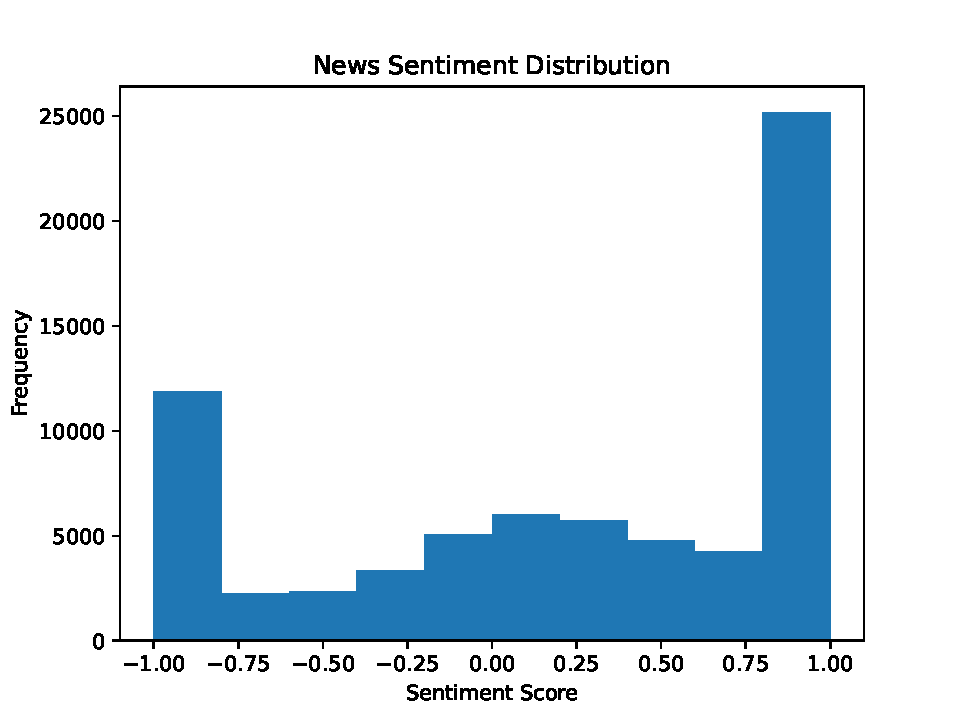
\includegraphics[width=.9\textwidth]{news_sent_dist}
\end{figure}

The figure highlights that news sentiment has a bimodal distribution. Much of the headlines are interpreted as either negative or positive, but news headlines that are relatively neutral, or closer to 0, or more evenly distriubuted. 
This indicates that the headlines that display strong enough sentiment that they could inform and change the actions of our reinforcement learning agents.



\section{Algorithmic and Analytical Challenge}

Our primary model technique is deep reinforcement learning, which is a 
branch of machine learning that operates in a game-theoretic-like system. 
Formally, a reinforcement learning problem is an instance of a Markov 
Decision Process, which is a 4-tuple $(S, A, T, R)$: $S$ the state space 
(matrix of selected historical stock price and news data available to 
our model at a given time; see Methodology section), $A$ the action space 
(portfolio weights produced by our model, under appropriate constraints), 
$T$ the transition function (how the state changes over time, modeled by our dataset), 
and $R$ (the reward function). The goal is to find a policy (function from $S \to A$) 
that maximizes future expected rewards. Most reinforcement learning research is 
spent on providing good information in $S$ to the model, defining a good reward 
function $R$, and deciding on a deep learning model training system to optimize rewards.

\subsection{Existing Literature}

Much of the literature applying RL to portfolio optimization has arisen in the 
last few years. Some relevant papers are:

\begin{itemize}

\item \cite{drl_mvo} Deep Reinforcement Learning Comparison with Mean-Variance Optimization: 
Using a lookback of recent past returns and a few market indicators 
(including 20-day volatility and the VIX), this paper implements a simple 
algorithm for portfolio weight selection to maximize the Differential Sharpe Ratio, 
a (local stepwise) reward function which approximates (global) Sharpe Ratio of the 
final strategy. They compare their model with the standard mean-variance 
optimization across several metrics.

\item \cite{drl_modern_portfolio_theory} DRL for Stock Portfolio Optimization Connected with Modern 
Portfolio Theory: This paper applies reinforcement learning methods to 
tensors of technical indicators and covariance matrices between stocks. 
After tensor feature extraction using 3D convolutions and tensor decompositions, 
the DDPG method is used to train the neural network policy, and the algorithm 
is backtested and compared against related methods.
 
\item \cite{rl_augmented_states} RL-Based Portfolio Management with Augmented Asset Movement Prediction 
States: The authors propose a method to augment the state space S of historical 
price data with embeddings of internal information and alternative data. 
For all assets at all times, the authors use an LSTM to predict the price movement,
which is integrated into S. When news article data is available, different NLP methods 
are used to embed the news; this embedding is fed into an HAN to predict price 
movement, which is also integrated into S for state augmentation. The paper applies 
the DPG policy training method and compares against multiple baseline portfolios on 
multiple asset classes. It also addresses challenges due to environment uncertainty, 
sparsity, and news correlations.

\item \cite{drl_framework} A Deep Reinforcement Learning Framework for the Financial Portfolio Management Problem: 
This paper contains a deep mathematical and algorithmic discussion of how to properly incorporate 
transaction costs into an RL model. The authors also have a GitHub with implementations of their 
RL strategy compared with several others.

\item \cite{learn_to_rank} Stock Portfolio Selection Using Learning-to-Rank Algorithms with News Sentiment: 
After developing news sentiment indicators including shock and trends, this paper applies 
multiple learning-to-rank algorithms and constructs an automated trading system with strong performance.

\item \cite{maps} MAPS: Multi-agent Reinforcement Learning-based Portfolio Management System: 
This paper takes advantage of reinforcement learning with multiple agents by defining a 
reward function to penalize correlations between agents, thereby producing multiple orthogonal 
(diverse) high-performing portfolios.

\end{itemize}

\subsection{Methodology}

We will be implementing, combining, and improving on the methodologies of several of the above papers. 
Our plan is to develop an RL system that utilizes multiple time periods to achieve strong out-of-sample 
trading performance. As of this writing, we have partial implementations of papers \cite{drl_mvo}, \cite{drl_modern_portfolio_theory}, and \cite{drl_framework}.
 Our final architecture will be most similar to papers \cite{rl_augmented_states} and \cite{drl_framework}.

\subsubsection{Markov Decision Process Problem Formulation}

Paper \cite{rl_augmented_states} includes the following diagram, which is very close to our desired 
architecture:

\begin{center}
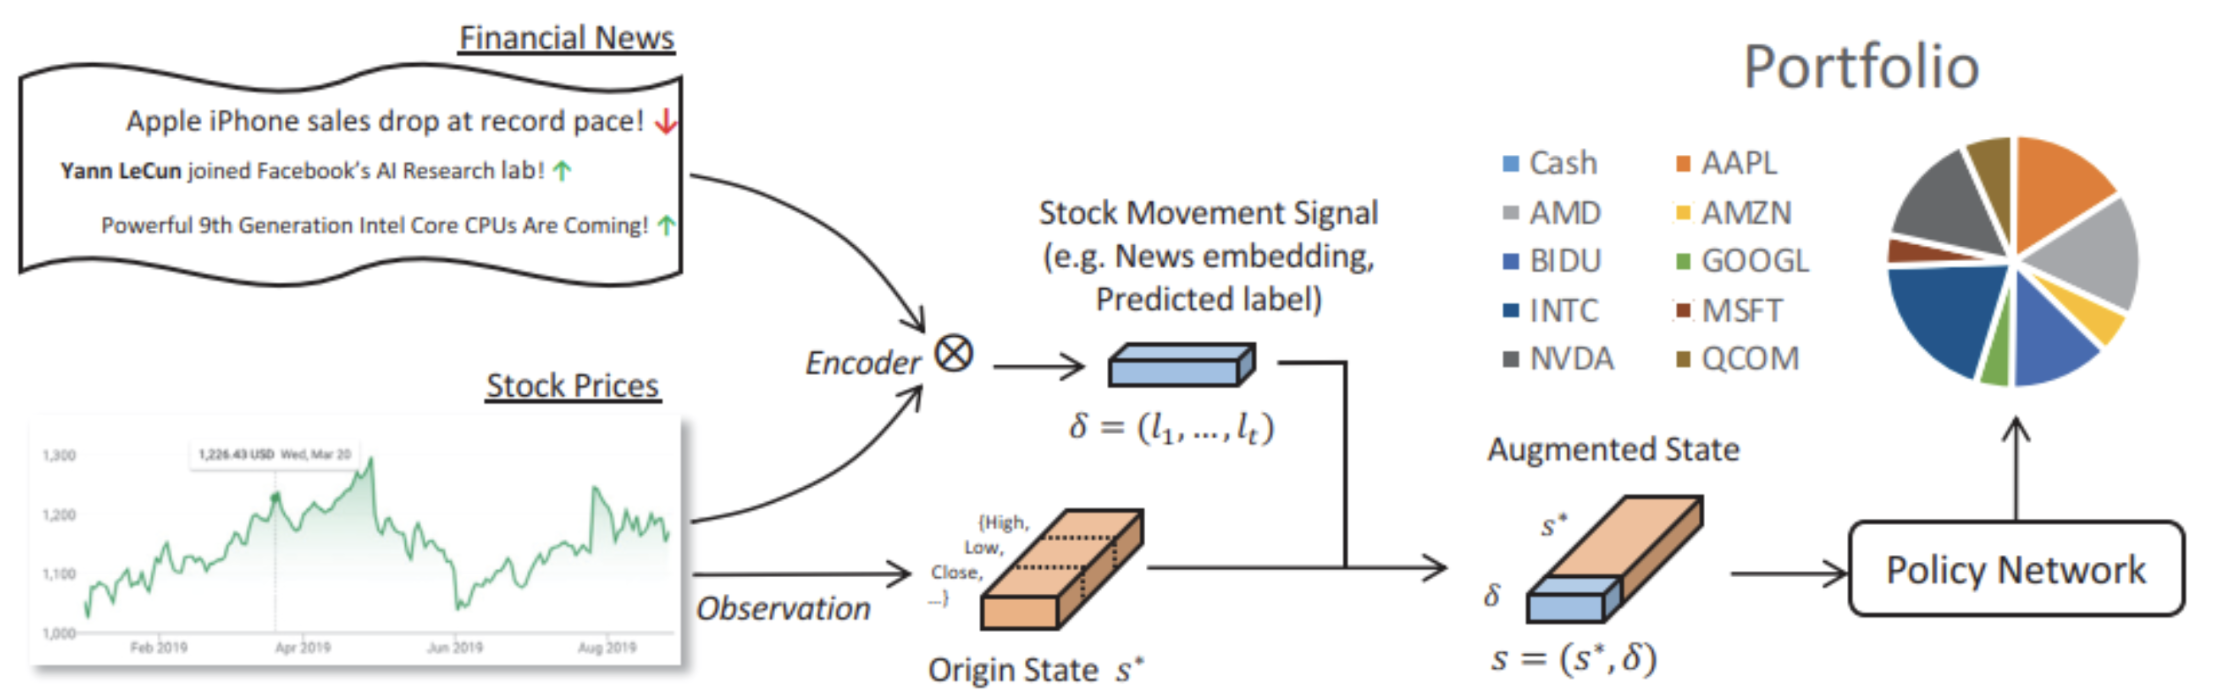
\includegraphics[width=13cm]{formulation.png}
\end{center}

An explanation of this diagram: at time t, the origin state $S^*$ is a 3D tensor of dimensions $U \times H \times C$
which contains historical price data. $U$ is the size of our universe (for example, for the S$\&$P100, $U = 100$). 
$H$ is the size of history we are providing (if we are providing 30 day history, then $H = 30$). 
$C$ is a categorical value representing the close/high/low price. This format of $S^*$ allows us to store, 
for example, the last 30 days of stock price data for all companies in the S$\&$P100, for any given day. 
In addition to this, we have news information $\delta$, obtained from financial news headlines for that day, 
processed through a pre-trained encoder. This information is added to $S^*$ to create the full state 
$S = (S^*, \delta)$

In our architecture, for $S^*$, we will experiment with the lookback period size and likely reduce it 
to a 2D array by flattening along the C index, but will otherwise keep $S^*$ largely the same. For 
$\delta$, we plan to utilize better feature extraction via sentiment scores and topic modeling; 
we also plan to use different alternative data sources, as described in the Dataset Creation section. 
In addition, we will extract what company each headline refers to, so our features can be changed 
over time independently for each company as news articles enter through our environment. The final 
state S will likely be a 2D matrix, where each row represents a different company (ticker), and along 
that row we find, concatenated, the following: (1) the past month-or-so of stock price data from $S^*$, 
and (2) numerical features extracted from recent news data pertinent to that company (as described 
in the Dataset section). (The straightforward concatenation of price data and news embeddings did not 
affect the ability of the neural network-based agent to learn.)

Regarding the reward function R, we plan to experiment with both the profit reward function used in \cite{rl_augmented_states}, 
as well as the Differential Sharpe Ratio developed in paper \cite{drl_mvo}.

In summary, our project aims to implement and replicate the approach used in \cite{rl_augmented_states}, with 
some modifications to S and R as previously described. We will conduct experiments alternative data 
sources, feature extraction methods, and reward functions (both custom and from other papers listed) 
to find a good combination that allows this approach to work well on S$\&$P100 stocks; this comprises our 
novel extension/contribution.

\subsubsection{Use of Libraries}

We will mainly be using the Gymnasium library to implement the reinforcement learning environments. 
The Stable Baselines 3 library provides several policy learning techniques that we will experiment with, 
including Proximal Policy Optimization (PPO) and Deep Deterministic Policy Gradients (DDPG). 
The papers above discuss the advantages and disadvantages of multiple reward functions and constraints, 
which we will make improvements upon and provide as options to the user, if applicable.

\subsubsection{Strategy Benchmarking}

Our final model architecture will be compared against several benchmark financial portfolio selection 
models. Among these will be the CAPM, an exponential moving average strategy, linear factor models 
such as the Fama French 3/5-factor models, and the QMJ model. We will compare our returns 
in-sample and out-of-sample plots, as well as our relative performance on portfolio statistics 
including cumulative return, Sharpe Ratio, Sortino Ratio, drawdown, etc. The experiment sections 
in the above papers provide a strong reference for our methodological comparison.



\chapter{Literature Notes and Commentary}

\section{Reinforcement Learning Overview}

The reader may not be readily familiar with reinforcement learning (RL).
Thus, we here provide a brief overview of the terminology, basic definition, essential results, and common algorithms in RL theory.

\subsection{Markov Decision Process}

A Markov Decision Process (MDP) problem is a framework for modeling sequential decision-making by an agent in an environment.
A problem is formally defined as a $4$-tuple $(S, A, T, R)$.
\begin{itemize}
  \item $S$ is the state space, which is the set of all possible states of the environment.
  \item $A$ is the action space, which contains all possible actions that the agent can take (across all possible states).
  \item $T: S \times A \times S \to [0, 1]$ is the transition function in a stochastic environment. When the environment is in state $s$ and
    the agent takes action $a$, then $T(s, a, s')$ is the probability that the environment transitions to state $s'$ as a result. (In a deterministic environment,
    this function may not be necessary, as there may be only one possible state due to the taken action.)
  \item $R: S \times A \times S \to \R$ is the reward function. When the environment changes state from $s$ to $s'$ due to action $a$, the agent recieves reward $R(s, a, s')$.
\end{itemize}
The environment is Markov, which means that the distribution of the next state $s'$ conditioned on the current state $s$ and action $a$ is independent from the time step.

A policy is a function $\pi: S \to A$ that dictates actions to take at a given state.
A solution to an MDP problem is an optimal policy $\pi^*$ that maximizes the agent's utility, however that is defined.

\subsection{RL Terminology}

In RL, the agent's utility is generally defined as the total expected discounted reward.
Let $\gamma \in [0, 1]$ be a constant discount factor. The utility from a sequence of reward $\{r_t\}_{t=0}^\infty$ is
thus commonly defined as $U([r_0, r_1, \ldots]) = \sum_{t=0}^\infty \gamma^t r_t \leq \frac{\sup_t r_t}{1-\gamma}$.
The benefit of this formulation is that (1) utility is bounded if the rewards are bounded, and (2) there is a balance
between small immediate rewards and large long-term rewards. (The use of the discount factor depends on the actual reward function.
For custom reward functions, it may not be necessary or even desireable; we include it because it is common in RL literature.)

Given a policy $\pi: S \to A$, we define the value function $V^\pi: S \to \R$ and the $Q$-function $Q^\pi: S \times A \to \R$ as
\begin{align*}
  V^\pi(s) = \E_\pi\left[ \sum_{t=0}^\infty \gamma^t R_t \:\Big|\: s_0 = s  \right] &&
  Q^\pi(s, a) = \E_\pi\left[  \sum_{t=0}^\infty \gamma^t R_t \:\Big|\: s_0 = s, a_0 = a \right]
\end{align*}
$V^\pi(s)$ is the expected utility from starting at $s$ and following policy $\pi$, and $Q^\pi(s, a)$ is the expected utility
from starting at $s$, taking action $a$, and then following policy $\pi$ thereafter.
The goal of RL is to find the optimal policy $\pi^*$, from which we have the optimal value function $V^*$ and optimal $Q$-function $Q^*$.
These optimal values can further be defined as follows:
\begin{align*}
  Q^*(s, a) &= \E_{s'}[R(s, a, s') + \gamma V^*(s')] = \sum_{s'} T(s, a, s')[R(s, a, s') + \gamma V^*(s')] \\
  V^*(s) &= \max_a Q^*(s, a) = \max_a \sum_{s'} T(s, a, s')[R(s, a, s') + \gamma V^*(s')]
\end{align*}
The second equation is known as the Bellman equation.

There are two main branches of RL: model-based and model-free.
In model-based RL, the agent attempt to build a model of the environment transition function $T$ and reward function $R$.
Based on these model, it then attempts to directly maximize the total expected reward.
In model-free RL, the agent does not attempt to model the environment, but instead attempts to learn either the value function or $Q$-function.
Once it has one of these, it can derive an optimal policy from it as:
\begin{align*}
  \pi^*(s) = \arg\max_a Q^*(s, a) = \arg\max_a \sum_{s'} T(s, a, s')\left[ R(s, a) + \gamma V^*(s')\right]
\end{align*}
We proceed with model-free RL in this project.

\subsection{Specialization to Our Application}

In the portfolio optimization setting, our RL agent seeks to produce an optimal set of portfolio weights given all the information it knows.
Assume that there are $n$ tradeable stocks in our universe, and one risk-free asset.
The action space $A = \left\{a \in \R^{n+1} \:|\: \sum_i a_i = 1\right\}$ is the set of all possible portfolio weights.

The state space $S$ encompasses all information available to the agent when it is asked to make a portfolio allocation decision at a given time.
Depending on what information is provided, this could include past performance of the strategy, historical stock prices, encoded news information for
select/all tickers in the universe, or some combination of these. For most of the scenarios we consider, $S \in \R^{n \times N}$ is a matrix, where
each row corresponds to a different stock ticker, and along that row we find the past few weeks of historical price data as well as some
aggregate of news sentiment indicators/scores.

The transition function $T$ is a delta function since state transitions are deterministic.
The environment uses the weights provided by the agent to reallocate the portfolio, computes the new portfolio value,
and reads in new historical stock data and news datapoints to form the next state (for the next time period) which is provided to the agent.
(The exact for of $T$ is not needed; it is implicitly defined by the deterministic environment udpates.)

The reward function $R$ should be such that it encourages the agent to produce good portfolio weights.
One simple reward function is pure profit: $R(s_t, a_t)$ is how much profit is gained to portfolio allocation $a_t$ during time interval $[t, t+1)$.
Another possible reward function is the Differential Sharpe ratio (as described in section \ref{diff_sharpe_ratio_section}), which urges the agent to make portfolio allocations to maximize its total Sharpe ratio. 



\section{Differential Sharpe Ratio}
\label{diff_sharpe_ratio_section}

\cite{drl_mvo} utilizes the Differential Sharpe Ratio to implement and evaluate a reinforcement learning agent.
The Differential Sharpe Ratio is based on Portfolio Management Theory, and is developed in the author' previous works \cite{diff_sharpe_ratio_paper} and \cite{diff_sharpe_ratio_book}.
We briefly review the theory developed in both sources.

The traditional definition of the Sharpe Ratio is the ratio of expected excess returns to volatility.
If $R_t$ is the return of the portfolio at time $t$, and $r_f$ is the risk-free rate then
\begin{align*}
  \mathcal{S} = \frac{\mathbb{E}_t[R_t] - r_f}{\sqrt{\Var_t[R_t]}}
\end{align*}

This works well to analyze a strategy once all data is collected.
The goal of traditional portfolio theory is to maximize the Sharpe Ratio over the given time period (equivalently,
to maximize the mean-variance utility function).

Unfortunately, this will not work for a reinforcement learning agent. The agent must be given a reward after every time step,
but the traditional Sharpe ratio is only calculated at the end.

The Differential Sharpe Ratio attempts to remedy this by approximating a change in the total Sharpe ratio up to that point.
By summing together many of these incremental changes (though approximate), the cumulative rewards is an approximation of the total
Sharpe ratio over the complete time period.

The approximation works by updating moment-based estimators of the expectation and variance in the Sharpe Ratio formula.
Let $A_t$ and $B_t$ be estimates of the first and second moments of the return $R_t$ up to time $t$.
After time step $t$, having obtained $R_t$, we perform the following updates:
\begin{align*}
  \Delta A_t = R_t - A_{t-1} && A_t = A_{t-1} + \eta \Delta A_t \\
  \Delta B_t = R_t - B_{t-1} && B_t = B_{t-1} + \eta \Delta B_t
\end{align*}
where $A_0 = B_0 = 0$ and $\eta \sim 1/T$ is an update parameter, where there are $T$ total time periods.
These updates are essentially exponential moving averages.

Let $S_t$ be an approximation of the Sharpe Ratio up to time $t$ based on estimates $A$ and $B$. That is,
\begin{align*}
  S_t = \frac{A_t}{\sqrt{B_t - A_t^2}}
\end{align*}
The definition here ignores the risk-free rate term. $K_\eta$ is a normalization constant to ensure an unbiased estimator.

Pretend that at the update for time $t$, $A_{t-1}$ and $B_{t-1}$ are constants,
and $R_t$ is also a known constant. Then the updates to $A_t$ and $B_t$ really only depend on the time step parameter $\eta$.
Indeed, if $\eta = 0$, then $A_t = A_{t-1}$ and $B_t = B_{t-1}$, so $S_t = S_{t-1}$.
Now consider varying $\eta$; expanding the Sharpe ratio estimator formula in Taylor series gives
\begin{align*}
  S_t \approx S_{t-1} + \eta \frac{\diff S_t}{\diff \eta}\Big|_{\eta = 0} + o(\eta^2)
\end{align*}

If $\eta$ is small, the final term is negligible, so this formula gives us an exponential-moving-average update for $S_t$.
The Differential Sharpe Ratio is defined to be proportional derivative in that expression. With some tedious calculus, we find that
\begin{align*}
  D_t &= \frac{\diff S_t}{\diff \eta} = \frac{\diff}{\diff\eta}\left[ \frac{A_t}{\sqrt{B_t - A_t^2}} \right] = \frac{\frac{\diff A_t}{\diff \eta} \sqrt{B_t - A_t^2} - A_t \frac{\frac{\diff B_t}{\diff \eta} - 2 A_t \frac{\diff A_t}{\diff \eta}}{2 \sqrt{B_t - A_t^2}}}{B_t - A_t^2} \\
  &= \frac{\Delta A_t \sqrt{B_t - A_t^2} - A_t \frac{\Delta B_t - 2 A_t \Delta A_t}{2 \sqrt{B_t - A_t^2}}}{B_t - A_t^2}
  = \frac{B_t \Delta A_t - \frac{1}{2} A_t \Delta B_t}{(B_t - A_t^2)^{3/2}}
\end{align*}

This reward function is simple to implement in an environment. The authors of the original papers provide
experimental support for the value of this reward function in a reinforcement learning setting.




\section{Transaction Costs}
\label{transaction_costs_section}

\cite{drl_framework} contains an excellent walkthrough of the mathematics for modeling transaction costs
in RL environment updates. We provide a shortened version here.

Suppose we have $m$ tradeable assets and the risk-free asset. Let $\mathbf v_t = (1, v_{1,t}, v_{2,t}, \ldots v_{m,t}) \in \R^{m+1}$ be the
prices of the assets at time $t$ (the first entry is the risk-free asset). The raw return vector is defined as
$\mathbf y_t = \mathbf v_t \varoslash \mathbf v_{t-1} \in \R^{m+1}$, where division is element-wise. Suppose the portfolio
weight vector during time period $t$ is $\mathbf w_t \in \R^{m+1}$, and let the value of the portfolio value at time $t$ be $p_t$.
If we were not considering transaction costs, then the portfolio return would be $\frac{p_t}{p_{t-1}} = \mathbf y_t \cdot \mathbf w_t$.

Unfortunately, buying and selling assets incurs transaction costs. Let $\mathbf w_t' \in \R^{m+1}$ be the effective portfoliio weights
at the end of time $t$ (it has changed from $\mathbf w_t$ due to the changes in price). We have
\begin{align*}
  \mathbf w_t' = \frac{\mathbf y_t \odot \mathbf w_t}{\mathbf y_t \cdot \mathbf w_t}
\end{align*}
where $\odot$ is element-wise multiplication. Between time $t-1$ and time $t$, the portfolio value is also
adjusted from $p_{t-1} \in \R$ to $p_t' = p_{t-1} \mathbf y_t \cdot \mathbf w_{t-1}$. Let $p_t$ be the value of the portfolio
after transaction costs, and let $\mu_t \in \R$ be the transaction cost factor, such that $p_t = \mu_t p_t'$.
We can keep track of the relevant time of each variable with the following diagram:

\begin{center}
  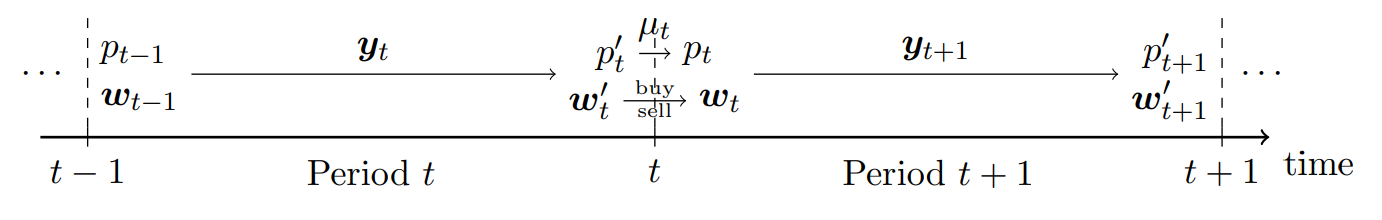
\includegraphics[width=13cm]{transaction_cost_time_updates.png}
\end{center}

In this paradigm, the final portfolio value at time $T$ is
\begin{align*}
  p_T = p_0 \prod_{t=1}^T \frac{p_t}{p_{t-1}} = p_0 \prod_{t=1}^T \mu_t \mathbf y_t \cdot \mathbf w_{t-1}
\end{align*}
The main difficulty is in determining the factor $\mu_t$, since it is an aggregate of all the transaction cost penalties.

Let $c_s \in [0, 1)$ be the commission rate for selling. We need to sell some amount of asset $i$ if 
there is more of asset $i$ in $\mathbf w_t'$ than in $\mathbf w_t$ by dollar value. Mathematically, this condition
is $p_t' w_{i,t}' > p_t w_{t,i}$, which is equivalent to $w_{i,t}' > \mu_t w_{i,t}$. Thus, the total amount of
money raised from selling assets is
\begin{align*}
  (1-c_s) p_t' \sum_{i=1}^m (w_{i,t}' - \mu_t w_{i,t})^+
\end{align*}
where $(\cdot)^+ = \max\{0, \cdot\} = \mathrm{ReLU}(\cdot)$. This money, as well as the money from adjusting the cash reserve
from $p_t' w_{0,t}'$ to $p_t w_{0,t}$, is used to purchase assets according to the opposite condition.
Let $c_p \in [0, 1)$ be the commision rate for purchasing. Equating the amount of money available from selling/cash and the amount of money
used for purchasing assets yields
\begin{align*}
  (1-c_p)\left[ w_{0,t}' - \mu_t w_{0,t} + (1-c_s) p_t' \sum_{i=1}^m (w_{i,t}' - \mu_t w_{i,t})^+ \right] = p_t'\sum_{i=1}^m (\mu_t w_{i,t} - w_{i,t}')+
\end{align*}
Moving terms around and simplifying the ReLU expressions, we find that $\mu_t$ is a fixed-point of the function $f$ defined as:
\begin{align*}
  \mu_t = f(\mu_t) = \frac{1}{1 - c_p w_{0,t}}\left[ 1 - c_p w_{0,t}' - (c_s + c_p - c_s c_p) \sum_{i=1}^m (w_{i,t}' - \mu_t w_{i,t})^+ \right]
\end{align*}
The function $f$ is a nonlinear. However, for reasonable values of $c_s$ and $c_p$, $f$ is both monotone increasing and a contraction, so its unique fixed point
can be found by iteratively computing values of $f$. This procedure is fairly efficient and easy to implement.


\chapter{Documentation}

\section{Gym Environments}

\section{AbstractPortfolioEnvWithTCost}

\begin{minted}{python3}
  WIP
  class AbstractPortfolioEnvWithTCost(gym.Env):
  def __init__(self, w_lb=0.0, w_ub=1.0, cp=0.0, cs=0.0, logging=True):
    # set constants
    self.eta = 1 / 252
    self.cp, self.cs = cp, cs
    self.logging = logging

    # get data, set problem size
    self.num_time_periods, self.universe_size = self.get_data()

    # set spaces
    assert w_lb <= w_ub
    self.observation_space = self.get_obs_space()
    self.action_space = gym.spaces.Box(
      low=w_lb,
      high=w_ub,
      shape=(self.universe_size + 1,),
      dtype=np.float32
    )

  @abstractmethod
  def get_obs_space(self) -> gym.spaces.Box:
    """Result is assigned to ``self.observation_space``"""
    pass

  @abstractmethod
  def get_data(self) -> tuple[int, int]:
    """
    This abstract function loads/fetches state data and stores it on the environment.
    This will be called during initialization. The properties assigned here should be
    accessed into the __compute_state() method. Note that the data should provide for
    one more than the number of time periods desired (for the initial state).
    :return: (number of time periods, number of stock tickers)
    """
    pass

  @abstractmethod
  def get_state(self) -> npt.NDArray[float]:
    """
    Computes and returns the new state at time ``self.t`` (to be used for
    calculating weights at the start of time period ``self.t+1``).
    When ``self.t == 0``, it should output the initial state.
    """
    pass

  @abstractmethod
  def get_prices(self) -> npt.NDArray[float]:
    """
    Obtains the security prices at time ``self.t`` (at the
    beginning of time period ``self.t+1``). When ``self.t == 0``, it
    should output the initial prices.
    """
    pass

  def initialize_reward(self):
    self.A, self.B = 0.0, 0.0

  def compute_reward(self) -> float:
    R = np.log(self.new_port_val / self.port_val)
    dA = R - self.A
    dB = R ** 2 - self.B
    if self.B - self.A ** 2 == 0:
        D = 0
    else:
        D = (self.B * dA - 0.5 * self.A * dB) / (self.B - self.A ** 2) ** (3 / 2)
    self.A += self.eta * dA
    self.B += self.eta * dB
    return D

  def find_mu(self, w_old: npt.NDArray[float], w_new = npt.NDArray[float]) -> float:
    cp, cs = self.cp, self.cs

    def f(mu: float) -> float:
        return ((1 - cp * w_new[-1] - (cs + cs - cs*cp) * (w_new[:-1] - mu * w_old[:-1]).clip(min=0).sum()) /
                (1 - cp * w_old[-1]))

    mu = 0.0
    for _ in range(30):
        mu = f(mu)
    return mu

  def step(self, action: npt.NDArray[float]) -> tuple:
    action = action / action.sum()
    self.w_new = action
    self.t += 1
    self.v_new = self.get_prices()
    self.y = self.v_new / self.v
    self.mu = self.find_mu(self.y * self.w / (self.y * self.w).sum(), self.w_new)
    self.new_port_val = self.port_val * self.mu * (self.y @ self.w)

    self.reward = self.compute_reward()

    self.state = self.get_state()
    self.w = self.w_new
    self.v = self.v_new
    self.port_val = self.new_port_val

    if self.logging:
      info = {
        'port_val': self.port_val
      }
    else:
      info = {}

    finished = (self.t == self.num_time_periods)
    return self.state.copy(), self.reward, finished, False, info

  def reset(self, *args, **kwargs) -> tuple[np.ndarray, dict]:
    # portfolio weights (final is cash weight)
    self.w = np.zeros(self.universe_size + 1, dtype=float)
    self.w[-1] = 1.0

    self.port_val = 1.0

    self.initialize_reward()

    # compute and return initial state
    self.t = 0
    self.state = self.get_state()
    self.v = self.get_prices()
    return self.state.copy(), {}
\end{minted}

\section{MPTWithTCost}

\begin{minted}{python3}
  WIP
  class MPTWithTCost(AbstractPortfolioEnvWithTCost):

    def get_obs_space(self) -> gym.spaces.Box:
        self.state_shape = (1, 1, 28, self.universe_size)
        self.t = 0
        self.get_indicators()
        return gym.spaces.Box(low=-np.inf, high=np.inf, shape=self.state_shape, 
        dtype=np.float64)
    
    def get_data(self) -> Tuple[int, int]:
        # read SNP data
        df = pd.read_csv('crsp_snp100_2010_to_2024.csv', dtype='string')
    
        # convert datatypes
        df = df[['date', 'TICKER', 'PRC', 'VOL', 'ASKHI', 'BIDLO', 'FACPR']]
        df.date = pd.to_datetime(df.date)
        df.FACPR = df.FACPR.fillna('0.0')
        df.astype({
            'PRC': float,
            'VOL': float,
            'ASKHI': float,
            'BIDLO': float,
            'FACPR': float
        })
    
        # drop duplicates and nans
        df = df.drop_duplicates(subset=['date', 'TICKER'])
        df.dropna(inplace=True)
    
        # only include stocks that are present in all dates
        ticker_ok = df.TICKER.value_counts() == df.TICKER.value_counts().max()

        def is_max_val_count(ticker: str) -> bool:
          return ticker_ok[ticker]
        
        ok = df.apply(lambda row: is_max_val_count(row['TICKER']), axis=1)
        df = df[ok]
        df = df[(df.date.dt.year >= 2010) & (df.date.dt.year <= 2019)]
    
        # create stock array
        self.stock_df = df.pivot(index='date', columns='TICKER', values='PRC').astype(float)
        
        idx_df = pd.read_csv('crsp_snpidx_2010_to_2024.csv', dtype={
          'DATE': 'string',
          'vwretd': float
        })
        idx_df.DATE = pd.to_datetime(idx_df.DATE)
        idx_df['vol_20'] = idx_df.vwretd.rolling(20).std()
        idx_df['vol_60'] = idx_df.vwretd.rolling(60).std()
        idx_df.set_index('DATE', inplace=True)
        self.idx_df = idx_df

        # adjust for stock splits
        facpr_df = df.pivot(index='date', columns='TICKER', values='FACPR').astype(float)
        self.stock_df = self.stock_df * (1+facpr_df).cumprod(axis=0)
        self.ret = np.log(self.stock_df.pct_change().iloc[1:, :] + 1)
        self.times = df.date.unique()[1:]
        self.tickers = df.TICKER.unique()

        return len(self.times)-28-1, len(self.tickers)

    def get_indicators(self):
        self.conv3d = torch.nn.Conv3d(in_channels=4, out_channels=32,
        kernel_size=(1, 3, 1), padding="same").to('cuda')
        self.relu = torch.nn.ReLU()
        self.tucker = Tucker(rank=self.state_shape, init="random")
        self.m = 28
        self.w1, self.w2, self.w3 = 28, 14, 9
        
        df = (pd.DataFrame(self.stock_df, columns=self.tickers))
        df = df.dropna()
        mp = {ticker: pd.DataFrame(df[ticker]).rename(columns={ticker: "close"})
         for ticker in self.tickers}
        # SMA df
        sma = {ticker: pd.DataFrame(mp[ticker].ta.sma(self.w1)).rename(
          columns={"SMA_28": ticker}) for ticker in self.tickers}
        sma_df = pd.concat(sma.values(), axis=1).fillna(0)
        # RSI df
        rsi = {ticker: pd.DataFrame(mp[ticker].ta.rsi(self.w2)).rename(
          columns={"RSI_14": ticker}) for ticker in self.tickers}
        rsi_df = pd.concat(rsi.values(), axis=1).fillna(0)
        # MACD df
        macd = {ticker: pd.DataFrame(mp[ticker].ta.macd(self.w3, 26, 12)["MACD_9_26_12"])
        .rename(columns={"MACD_9_26_12": ticker}) for ticker in self.tickers}
        macd_df = pd.concat(macd.values(), axis=1).fillna(0)

        # Compute F = V @ Corr
        V = np.array([np.array(x.T) for x in [df, sma_df, rsi_df, macd_df]])
        Corr = np.array([np.corrcoef(x) for x in V])
        self.F = torch.from_numpy(np.einsum('aki,akj->akij', V, Corr)).to('cuda').float()


    def get_state(self) -> npt.NDArray[np.float64]:
        f = self.F[:, :, self.t + 28 - self.m : self.t + 28, :].clone().detach()      
        f = torch.unsqueeze(f, dim=0) 
        f = self.conv3d(f)
        f = self.relu(f)
        f = torch.squeeze(f, dim=0)
        f = f.cpu()
        core, _ = self.tucker.fit_transform(f)
        return core.detach().numpy()

    def get_prices(self) -> npt.NDArray[np.float64]:
        return np.append(self.stock_df.loc[self.times[self.t+28], :].to_numpy().
        flatten(), 1.0)
    
\end{minted}


\addcontentsline{toc}{chapter}{Bibliography}
\bibliographystyle{unsrtnat}
\bibliography{papers}


\end{document}